\documentclass[11pt]{article}

\usepackage[margin=1in]{geometry}
\usepackage[T1]{fontenc}
\usepackage{lmodern}
\usepackage{microtype}
\usepackage{amsmath,amssymb,amsthm,mathtools}
\usepackage{graphicx}
\usepackage[dvipsnames]{xcolor}
\usepackage{booktabs}
\usepackage{hyperref}

\hypersetup{
  colorlinks=true,
  linkcolor=MidnightBlue,
  citecolor=MidnightBlue,
  urlcolor=MidnightBlue
}

\newtheorem{theorem}{Theorem}
\newtheorem{proposition}{Proposition}
\newtheorem{remark}{Remark}

\newcommand{\E}{\mathbb{E}}
\newcommand{\Tmax}{T}

\title{\textbf{Eliminative Information in a Generalized Monty Hall Problem III}\\
\large Heterogeneous Rewards and Strategic Initial Choice}
\author{}
\date{}

\begin{document}
\maketitle

\begin{abstract}
Parts I and II studied identical rewards.  This note introduces heterogeneous
nonnegative rewards.  There are two distinct cases.  If reward labels are
exchangeable, then heterogeneity is mostly harmless: under uniform switching,
the expected reward after $t$ reveals depends only on total reward mass
$V=\sum_i v_i$.  If door labels carry different prior reward distributions,
the problem changes qualitatively.  The identity of Monty's zero-reward
reveals matters, switching rules diverge, and the initial door can become a
strategic sacrifice: choosing a low-prior door can preserve high-prior doors
for later switching.
\end{abstract}

\section{Two Kinds of Heterogeneity}

Heterogeneous rewards can mean two different things.

\paragraph{Exchangeable rewards.}
There is a multiset
\[
  \{v_1,\dots,v_m,0,\dots,0\},
\]
randomly permuted among $K$ doors.  Door labels carry no information.

\paragraph{Door-specific priors.}
Each door $j$ has its own prior distribution for a nonnegative reward $X_j$.
The player knows these priors but not the realized rewards.  Monty observes
the realized rewards and may reveal only zero-reward doors.

The first model gives a clean theorem.  The second model is where the new
decision theory appears.

\section{Exchangeable Reward Multisets}

Let positive rewards $v_1,\dots,v_m$ be randomly placed among $K$ doors, along
with $K-m$ zeros.  Let
\[
  V=\sum_{i=1}^m v_i.
\]
The player chooses an initial door uniformly.  Monty reveals $t$ zero-reward
doors, never opening the initial door.  The player then switches uniformly
among the remaining non-initial closed doors.

\begin{theorem}[Collapse to total reward mass]
Under exchangeable placement and uniform switching,
\[
  \E[\text{stay reward}]=\frac{V}{K}
\]
and
\[
  \E[\text{switch reward after }t\text{ reveals}]
  =
  \frac{V(K-1)}{K(K-1-t)}.
\]
\end{theorem}

\begin{proof}
The expected reward of the initial door is $V/K$ by exchangeability.  The
total expected reward mass outside the initial door is $V(K-1)/K$.  Monty
reveals only zero-reward doors, so this reward mass is not changed by the
reveals.  After $t$ reveals it is spread symmetrically over $K-1-t$ switch
options.  Uniform switching therefore has expected reward
\[
  \frac{1}{K-1-t}\cdot\frac{V(K-1)}{K}
  =
  \frac{V(K-1)}{K(K-1-t)}.
\]
\end{proof}

\begin{figure}[ht]
  \centering
  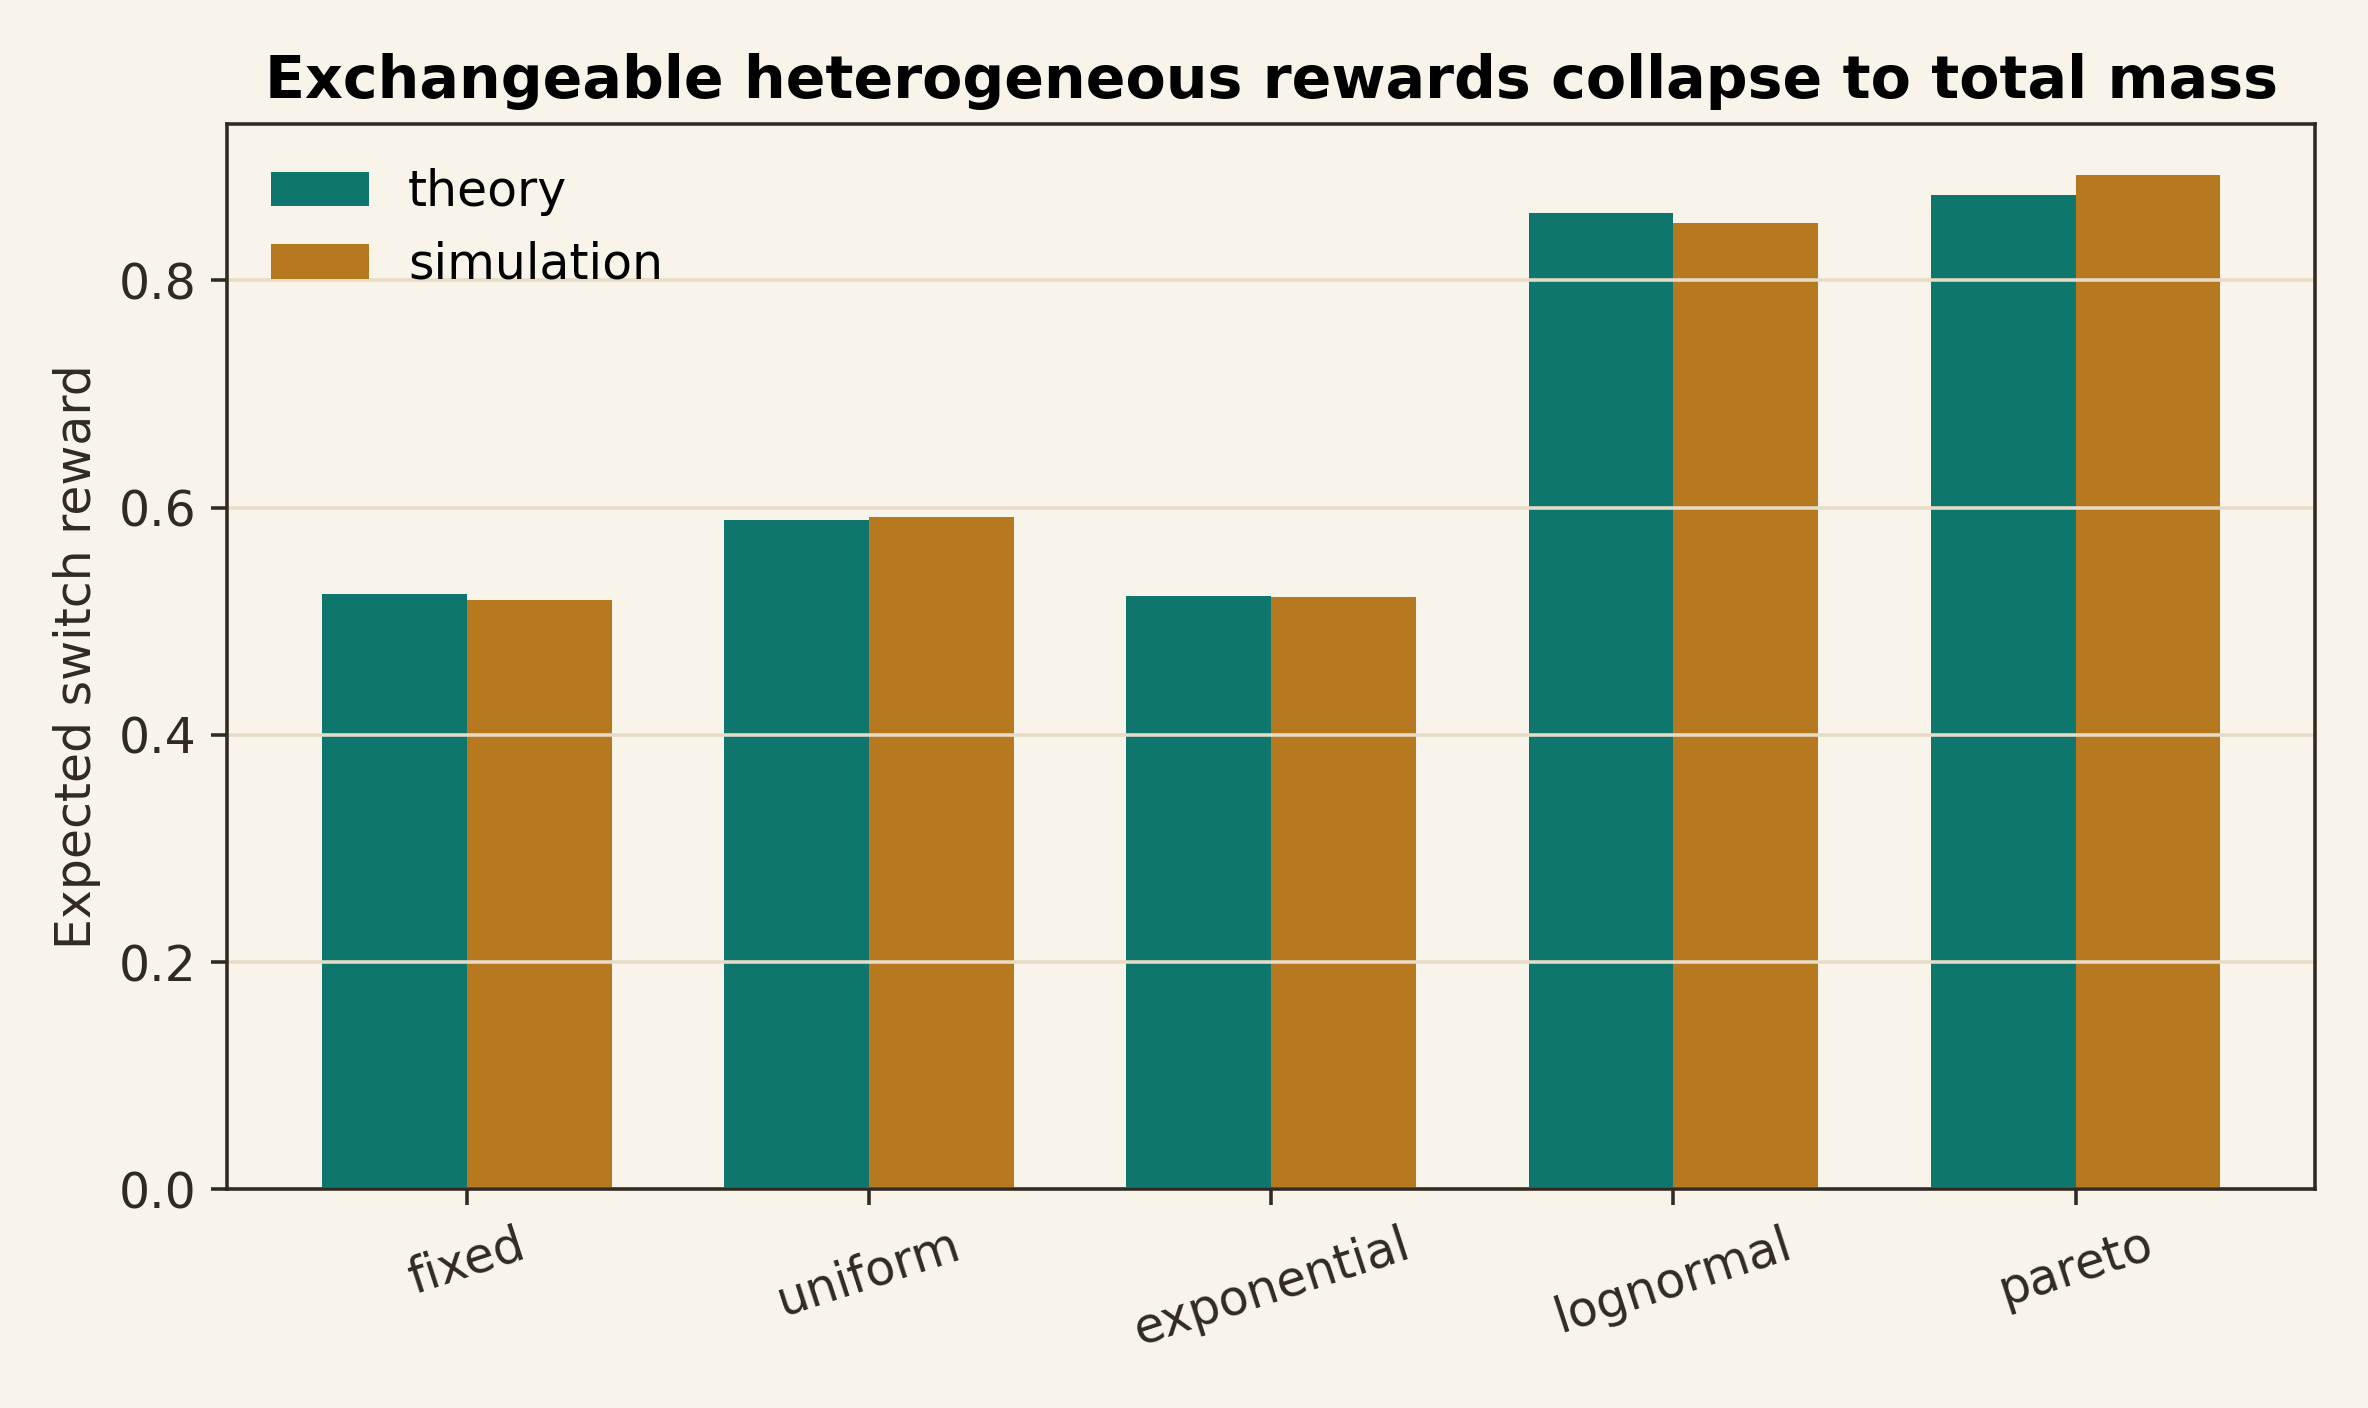
\includegraphics[width=0.88\linewidth]{fig_exchangeable_collapse.png}
  \caption{For exchangeable reward multisets, simulations match the total-mass
  formula across several reward distributions.}
  \label{fig:exchangeable}
\end{figure}

\begin{remark}
If all positive rewards are unit rewards, then $V=m$ and this reduces to the
Part I formula.  Heterogeneity alone does not complicate the model.  Labeled
asymmetry does.
\end{remark}

\section{Door-Specific Bernoulli-Value Priors}

For a first labeled model, let each door have
\[
  X_j =
  \begin{cases}
  0, & \text{with probability } q_j,\\
  v_j, & \text{with probability } 1-q_j.
  \end{cases}
\]
The prior mean is
\[
  \mu_j=(1-q_j)v_j.
\]
This model has a real atom at zero, so Monty has legal zero-reward doors to
reveal.  It also makes door labels meaningful.

\begin{figure}[ht]
  \centering
  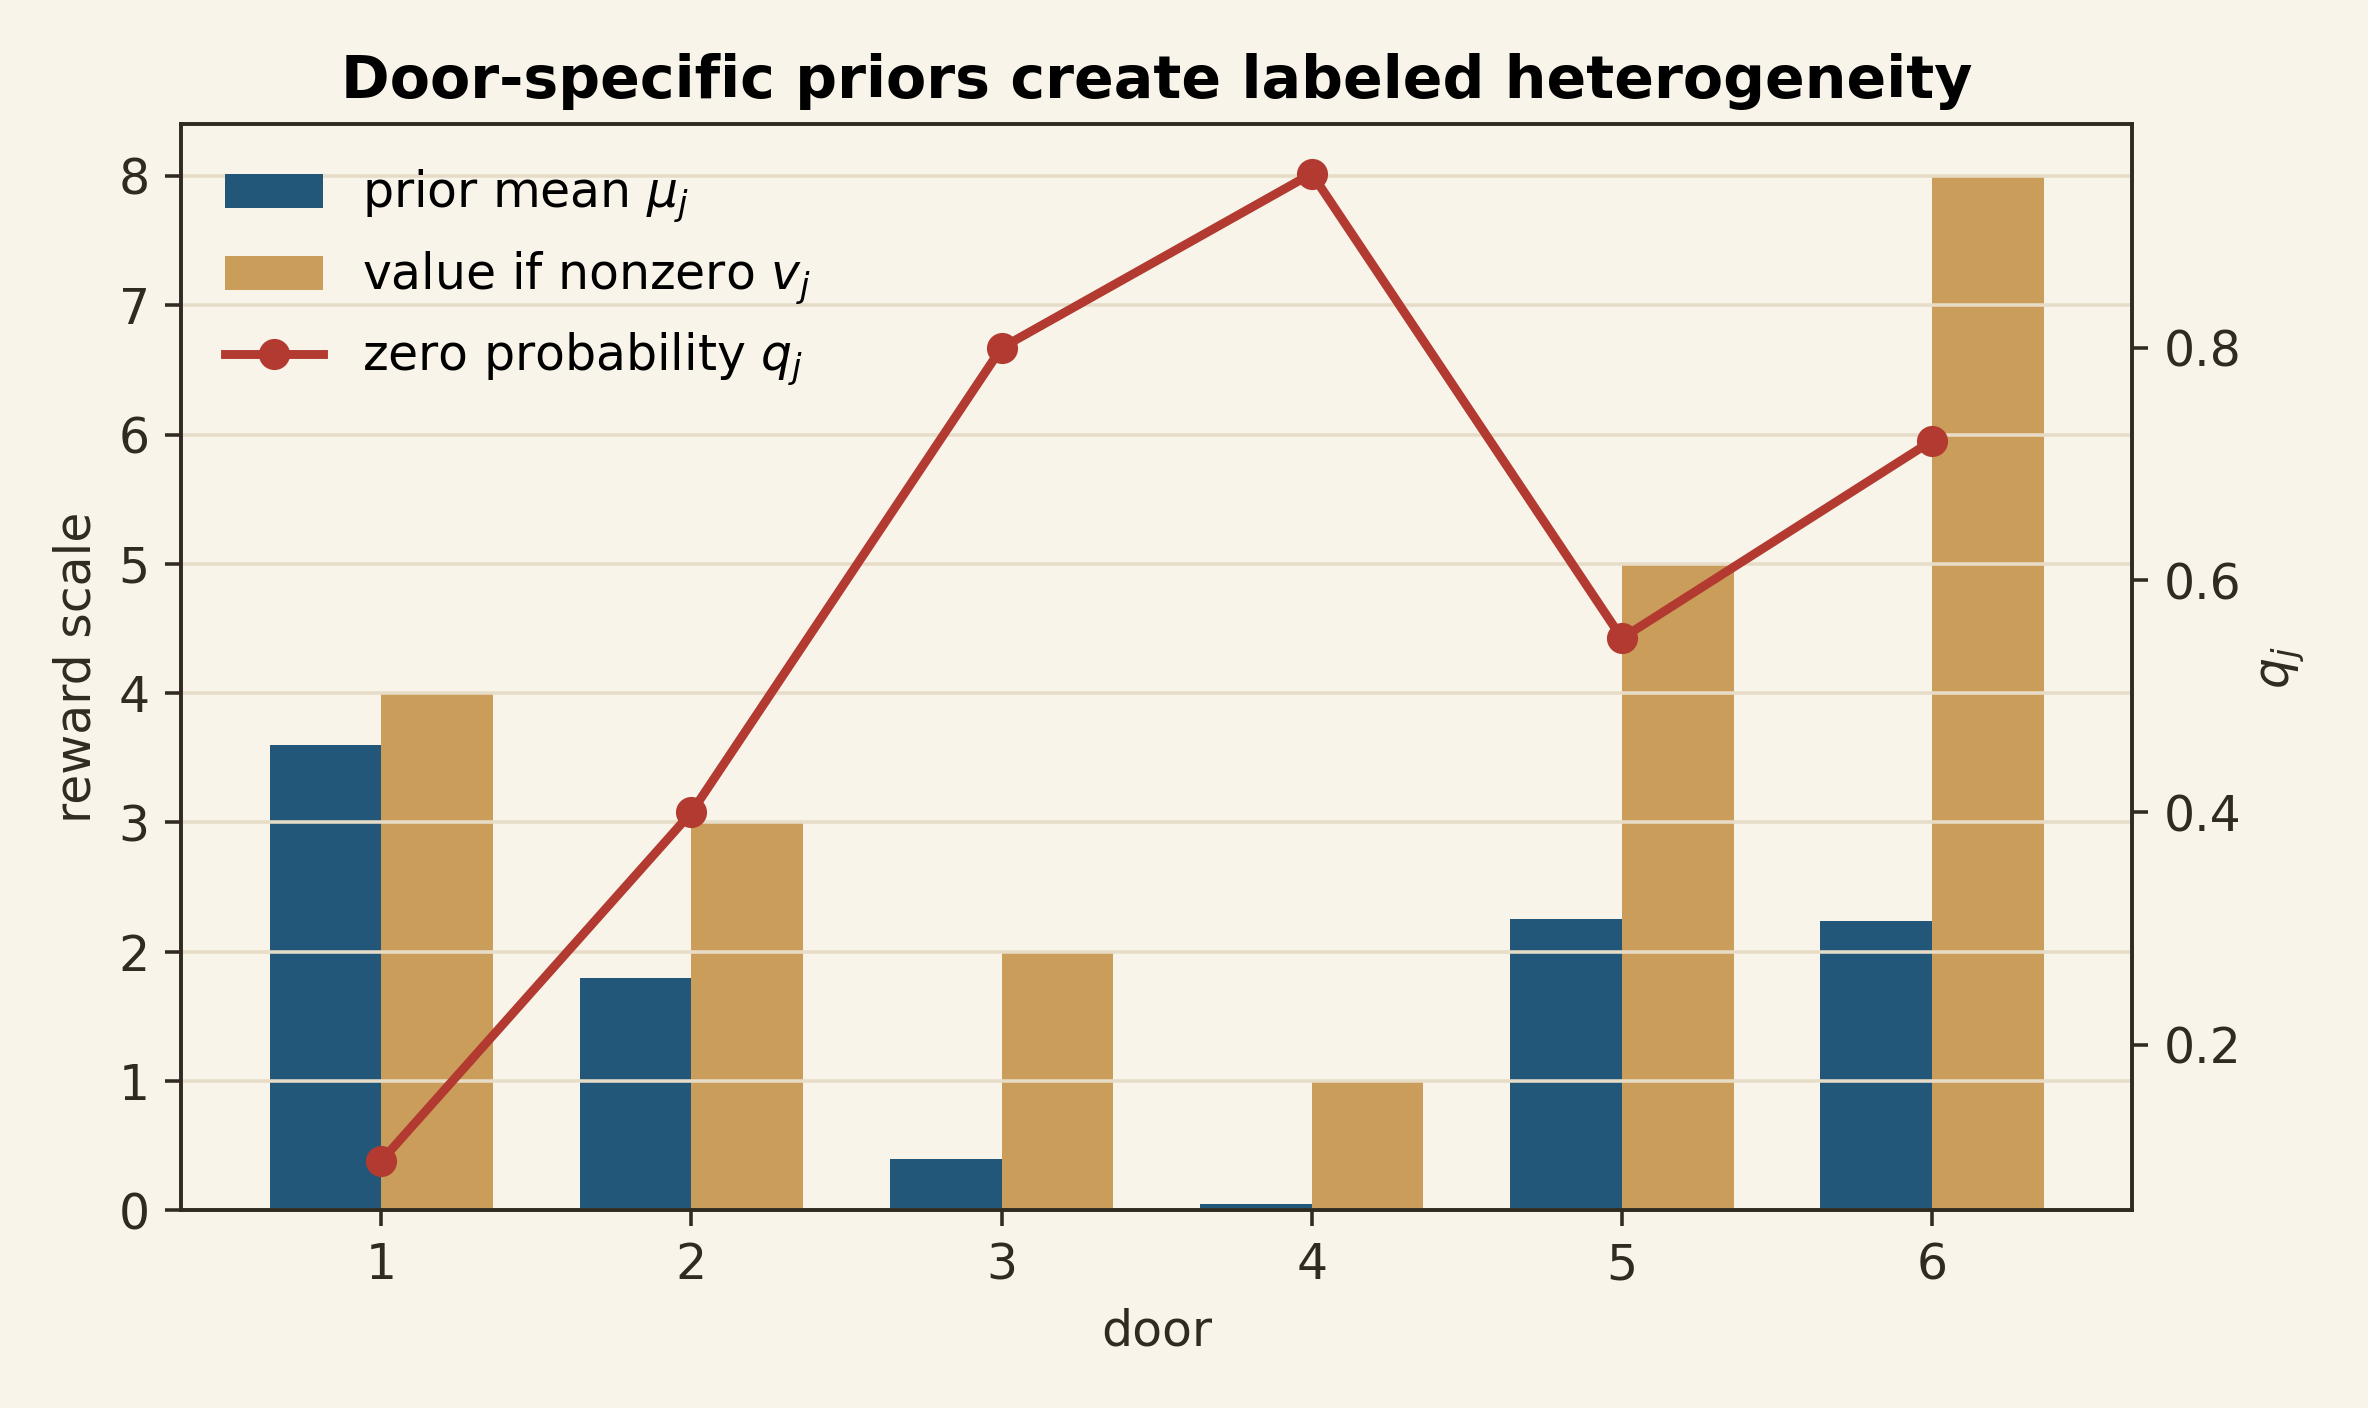
\includegraphics[width=0.88\linewidth]{fig_prior_landscape.png}
  \caption{A labeled prior landscape: doors differ in zero probability,
  positive reward size, and prior mean.}
  \label{fig:prior-landscape}
\end{figure}

\section{Switching Rules Separate}

With exchangeable doors, uniform switching is natural.  With labeled priors,
several switch rules differ:

\begin{itemize}
\item stay with the initial door;
\item switch uniformly among available doors;
\item switch to the available door with largest prior mean $\mu_j$;
\item switch to the available door with largest realized reward, an oracle
upper bound.
\end{itemize}

\begin{figure}[ht]
  \centering
  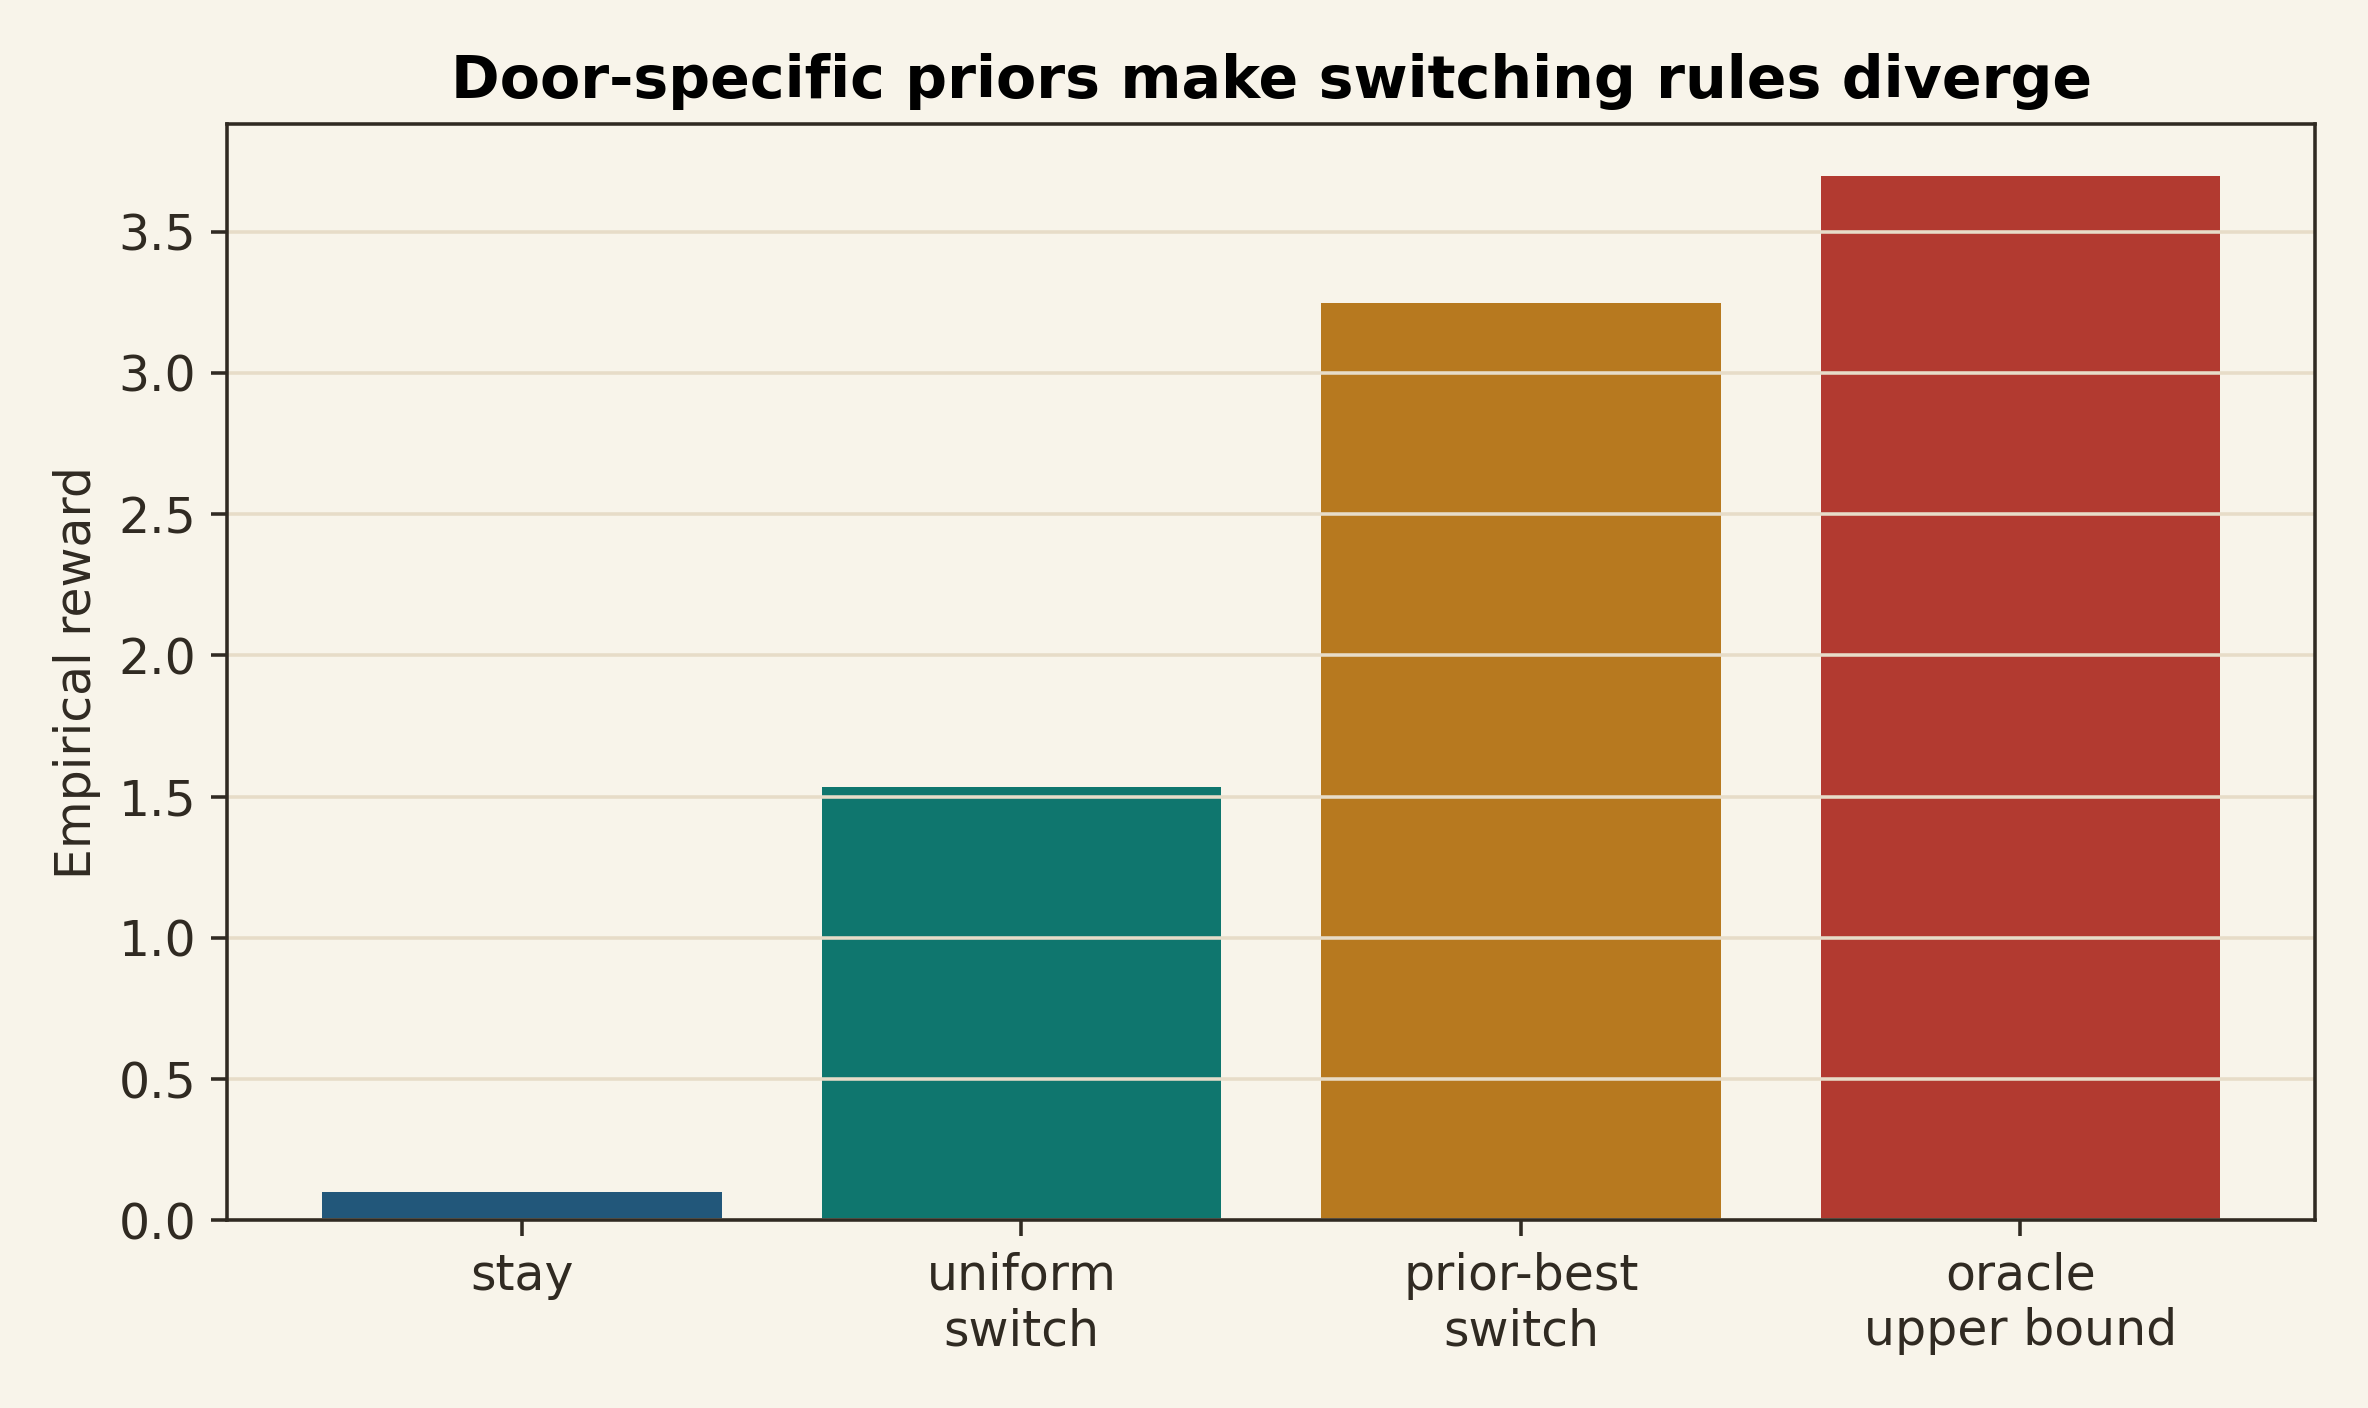
\includegraphics[width=0.88\linewidth]{fig_strategy_comparison.png}
  \caption{With door-specific priors, prior-best switching can substantially
  outperform uniform switching.  The oracle bar is an infeasible upper bound.}
  \label{fig:strategies}
\end{figure}

\section{Strategic Initial Choice}

The initial choice is irrelevant in the symmetric model.  It is not irrelevant
with labeled priors.  If the player expects to switch, choosing a high-mean
door initially can be wasteful because that door is removed from the switch
set.  Choosing a low-mean door can preserve high-mean doors for later.

\begin{proposition}[Sacrifice choices can be valuable]
There exist door-specific priors for which choosing the lowest-mean door as
the initial door gives a larger expected prior-best switch reward than choosing
the highest-mean door.
\end{proposition}

\begin{proof}
The claim is constructive.  Consider four doors with Bernoulli-value priors
\[
\begin{array}{c|cccc}
j & 1 & 2 & 3 & 4\\
\hline
q_j & 0.10 & 0.40 & 0.80 & 0.95\\
v_j & 4.00 & 3.00 & 2.00 & 1.00
\end{array}
\]
so that the prior means are $3.6,1.8,0.4,0.05$.  If the player chooses door
1 initially, the best switch candidates exclude the highest-mean door.  If
the player chooses door 4 initially, doors 1 and 2 remain available for
switching.  Direct enumeration or simulation under uniform zero-revealing
Monty shows that the latter policy has the larger prior-best switch reward.
Figure~\ref{fig:sacrifice} displays the comparison.
\end{proof}

\begin{figure}[ht]
  \centering
  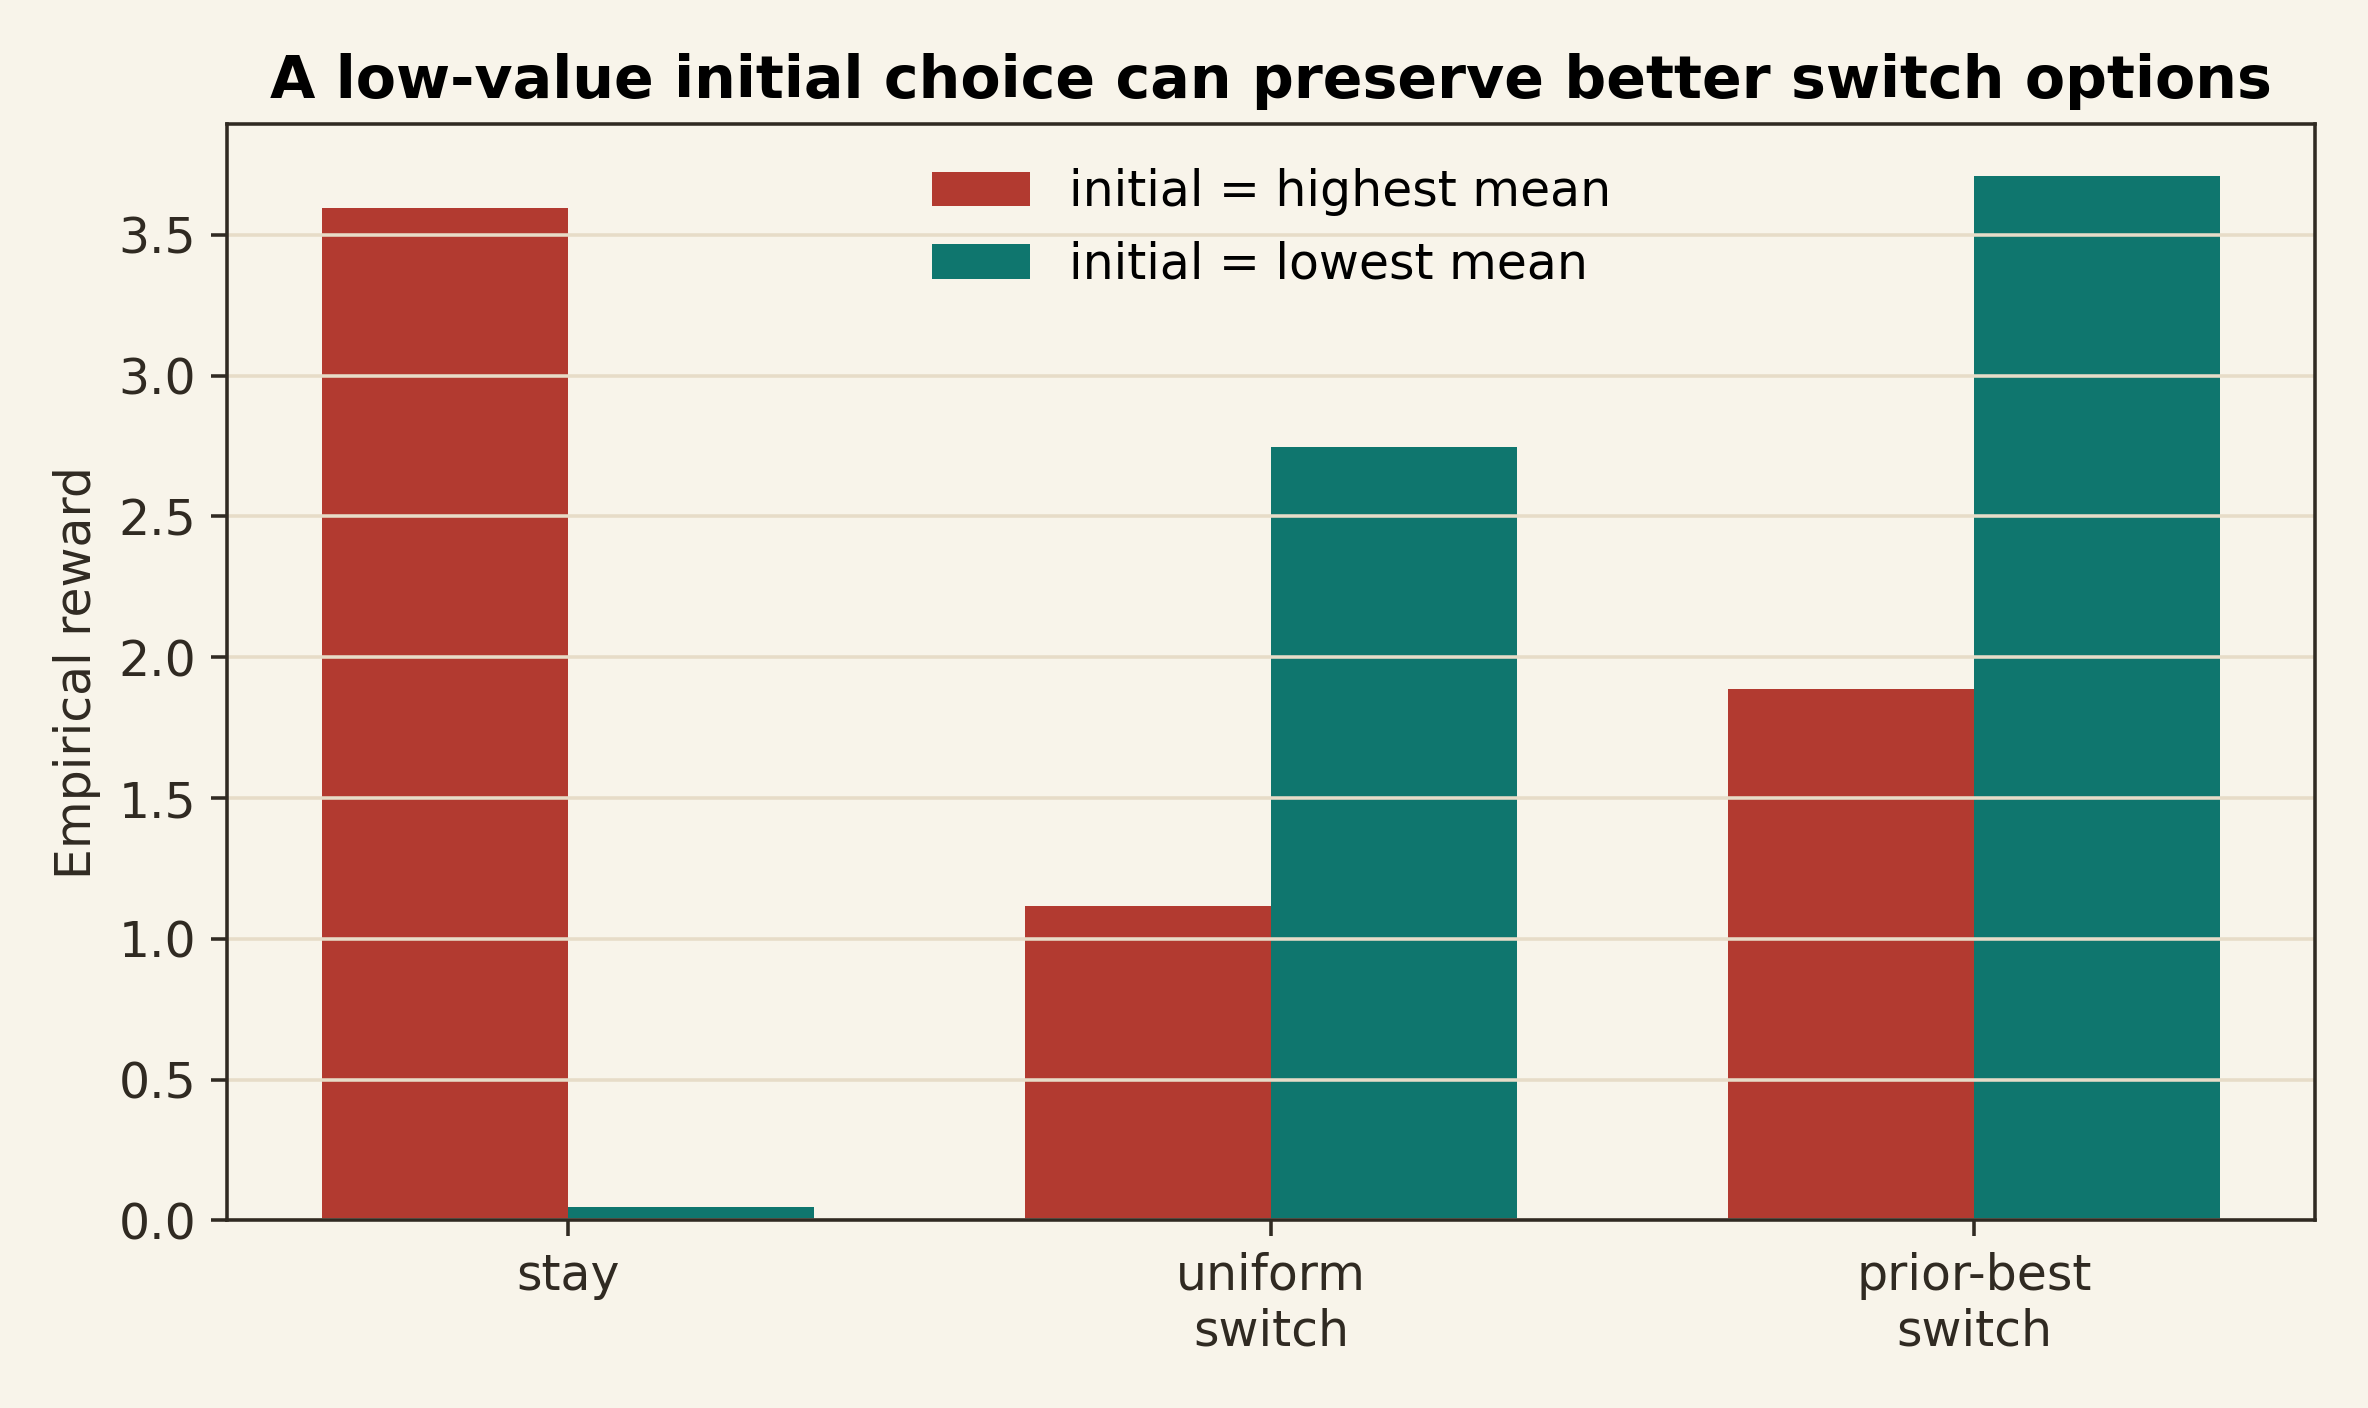
\includegraphics[width=0.88\linewidth]{fig_sacrifice_choice.png}
  \caption{A low-value initial choice can preserve better switch options.}
  \label{fig:sacrifice}
\end{figure}

\section{Monty's Policy Now Matters}

In the symmetric model, Monty's choice among legal zero doors is irrelevant.
With labeled priors, it matters.  Revealing a zero door with high prior mean is
more informative than revealing a zero door that was already expected to be
empty.

\begin{figure}[ht]
  \centering
  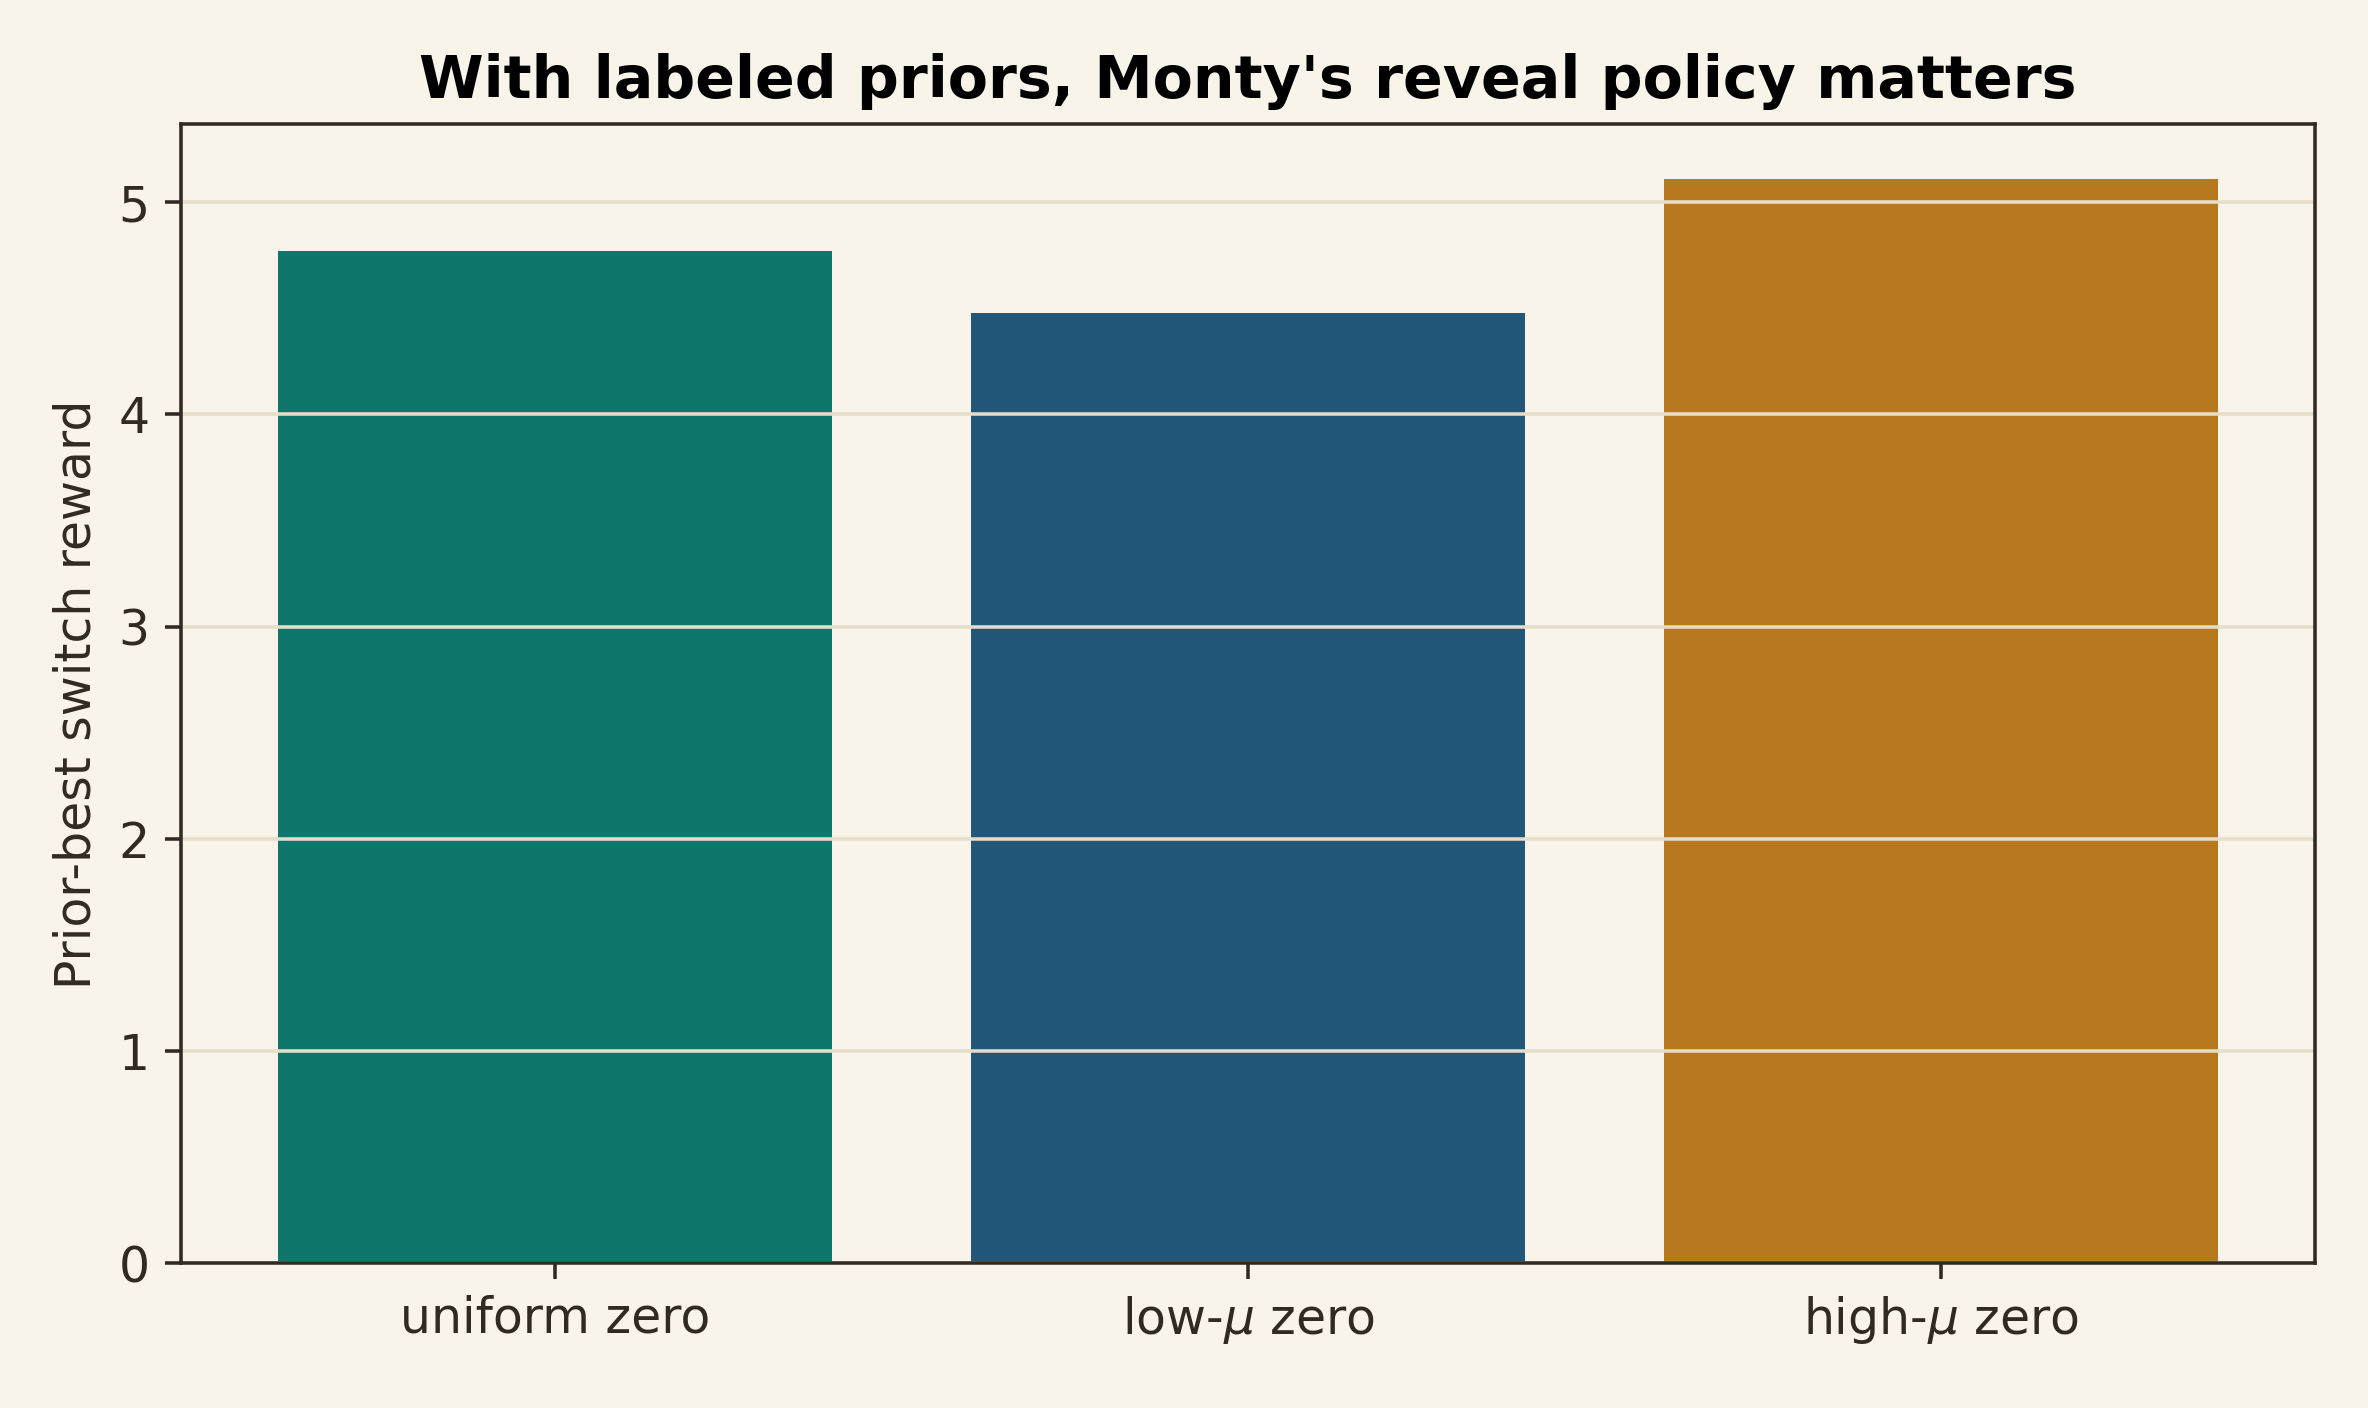
\includegraphics[width=0.88\linewidth]{fig_monty_policy_effect.png}
  \caption{Different legal reveal policies can change the value of prior-best
  switching.  This is the first point where host behavior becomes genuinely
  strategic.}
  \label{fig:monty-policy}
\end{figure}

\section{Concrete Numerical Examples}

The simulations above are meant as illustrations, but several numerical
examples are especially revealing.

\paragraph{Exchangeable rewards remain scalar.}
With $K=12$, $m=4$, $t=4$, and Pareto-distributed positive rewards, a run with
50,000 trials gave mean total reward
\[
  \bar V \approx 6.685.
\]
The empirical and theoretical values were:
\[
\begin{array}{lcc}
\toprule
\text{strategy} & \text{empirical reward} & \text{theory}\\
\midrule
\text{stay} & 0.5549 & 0.5571\\
\text{uniform switch} & 0.8774 & 0.8754\\
\bottomrule
\end{array}
\]
Even with heavy-tailed positive rewards, the exchangeable model behaves just
as the theorem predicts.  The individual reward distribution is not the main
source of complexity; labeled information is.

\paragraph{Door-specific priors create large strategy gaps.}
In a door-specific Bernoulli-value model with $K=10$, $t=2$, random priors, and
the lowest-mean door chosen initially, one run produced:
\[
\begin{array}{lc}
\toprule
\text{strategy} & \text{empirical reward}\\
\midrule
\text{stay} & 0.073\\
\text{uniform switch} & 0.585\\
\text{prior-best switch} & 1.373\\
\text{oracle switch} & 1.662\\
\bottomrule
\end{array}
\]
The prior-best strategy captures most of the oracle upper bound, while uniform
switching leaves substantial value on the table.  This is the practical
meaning of door-specific priors: once doors have different expected values,
``switch'' is no longer a single strategy.

\paragraph{The sacrifice effect can be dramatic.}
A search over four-door Bernoulli-value prior instances found the following
door priors:
\[
\begin{array}{c|ccc}
j & q_j & v_j & \mu_j=(1-q_j)v_j\\
\hline
1 & 0.256 & 2.745 & 2.042\\
2 & 0.642 & 2.390 & 0.855\\
3 & 0.329 & 28.833 & 19.342\\
4 & 0.230 & 0.450 & 0.347
\end{array}
\]
Door 3 is overwhelmingly the best door by prior mean.  If the player chooses
the highest-mean door initially, then that door is unavailable as a switch
target.  If the player instead chooses the lowest-mean door initially, the
high-value door remains available for switching.

The resulting empirical rewards were:
\[
\begin{array}{lcc}
\toprule
\text{strategy} & \text{initial = highest mean} & \text{initial = lowest mean}\\
\midrule
\text{stay} & 19.220 & 0.344\\
\text{uniform switch} & 1.439 & 10.028\\
\text{prior-best switch} & 2.245 & 19.729\\
\text{oracle switch} & 2.328 & 20.023\\
\bottomrule
\end{array}
\]
This is the clearest numerical expression of the new phenomenon.  In the
classical problem the initial choice is a guess.  Here it can be an
instrument.  If the plan is to switch, the player may rationally choose a bad
initial door in order to preserve the best doors for the switch set.

\section{Conclusion}

Heterogeneous rewards split the theory into two regimes.  Under exchangeable
placement and uniform switching, the problem remains scalar: only total reward
mass matters.  Under door-specific priors, the problem becomes a labeled
decision problem.  The identity of revealed zero doors matters, switching
rules separate, Monty's policy matters, and the initial choice can rationally
be a sacrifice.  This is the natural starting point for posterior updating and
fully strategic host models.

\end{document}
